\section{Algorithm-Dictated Incentives}
When decision-makers determine our access to things we want (loans, college admissions, etc.), we inevitably wonder what we can do to make them more likely to decide in our favor. In an increasingly data-driven world, it is common for decision-makers to train machine-learning models to automate the decision-making process. These machine-learning-based decision methods are generally designed to maximize the accuracy of their predictions, without considering how the decision process might affect subjects' behavior.
Yet, such models do implicitly define incentives to those subjected to their decisions, with serious social consequences. 

Consider a variant of an example raised by \citet{eubanks_2018}: families in distress are both more likely to utilize public welfare programs (such as food aid and public housing) and separately more likely to default on their debt. A model trained to predict creditworthiness would, in turn, learn a correlation between utilizing aid and failure to repay. Thus, struggling parents may need to avoid using vital aid for fear they would be denied a loan in their time of need, further exacerbating a family's deprivation.

% For a joke example in future presentations:
% \yocomment{
% Decision processes generate unintended incentives in many far more mundane tasks. 
% In a hypothetical setting, researchers submitting work to top machine learning conferences may know that paper acceptance is highly stochastic (with one program committee rejecting $57\%$ of another program committee's acceptances \cite{price_2014}). This incentivizes crafty authors with rejected papers to resubmit the same paper next year with few changes, hoping they get lucky while doing no extra work, instead of putting in further work to improve the paper.\footnote{Not that this is happening.}}
In this work, we propose a framework for studying the incentives defined by black-box decision functions, including nonlinear functions like neural networks and random forests, given only query access to the function. To the best of our knowledge, our work is the first to propose a definition for the incentives induced by arbitrary black-box decision functions, and to propose a method for determining the actions these decisions incentivize.

First, let us clarify terms. There exists a \textit{decision-maker}, who will at some point in the future make a decision about an individual, referred to as a \textit{decision subject}, based on that individual's \textit{state}. We say that this subject has \textit{agency} if they are capable of taking \textit{actions} to change their state, and thus affect the decision they will ultimately receive. An \textit{advice policy} is a recommendation for which actions to take at each state. By encouraging some actions over others, a decision-maker provides \textit{incentives} to individuals. The \textit{maximally-incentivized action} will, if executed, result in a better final decision than any alternative action.

While identifying an incentivized action from a given decision rule may seem straightforward, it can require surprising nuance. Consider the bimodal decision function in Figure \ref{fig:1di}. Whether the individual is "incentivised" to move left or right depends not only on the decision rule itself, but also how many resources (e.g. time, money) the individual has to expend on future actions.
\begin{figure}
    \centering
\minipage{0.38\textwidth}
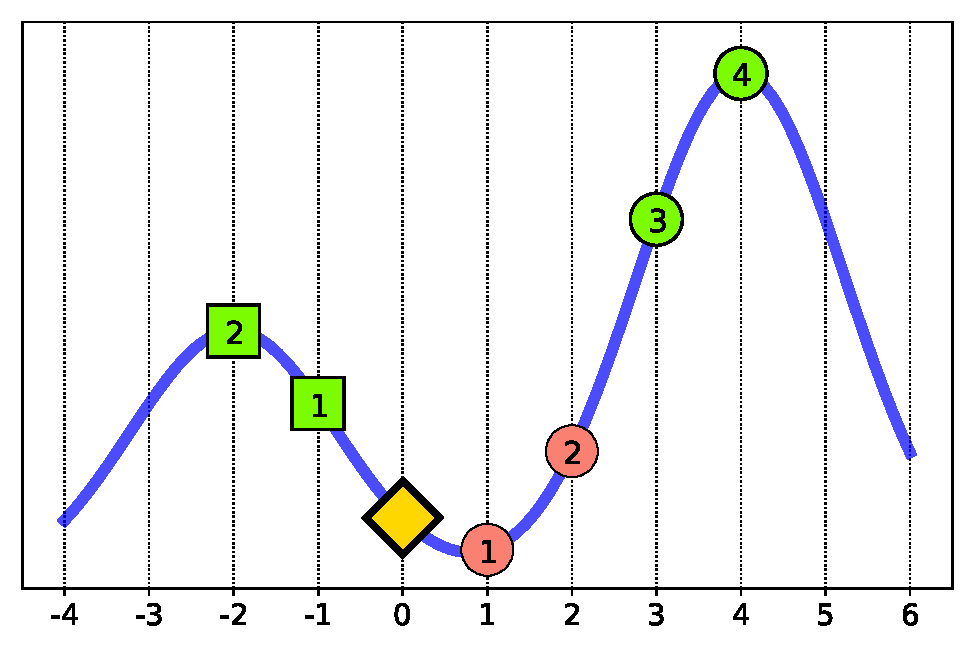
\includegraphics[width=\linewidth]{figures/incentive_1d.pdf}
\endminipage\hfill
\minipage{0.58\textwidth}
    \caption{A subject (gold diamond) wants to maximize the decision received from a decision rule (blue line) by stepping right or left, or staying in place. Each step expends 1 resource (e.g. time, money). The decision is only made when all the resources are used up, or the individual has stopped. If the individual has two resources or fewer, they should head towards the left peak (squares). On the other hand, if they have 3 resources or more, they should move right, because even though their interim state may seem worse, their final decision will be better (circles).}
\endminipage

    \label{fig:1di}
\end{figure}

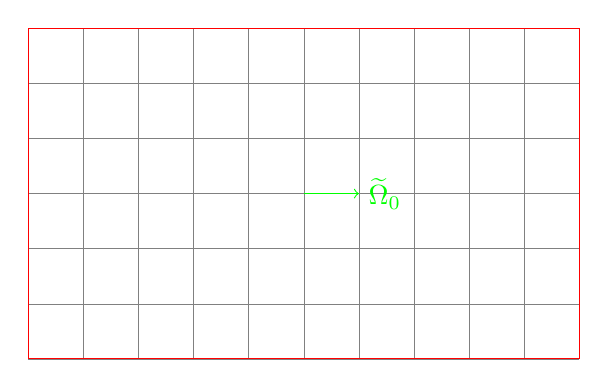
\begin{tikzpicture}[scale=0.7]

\draw[style=help lines] (0,0) grid (10,6);

\draw[red] (0,0) -- (10,0) -- (10,6) -- (0,6) -- (0,0);

\draw[green, ->] (5,3) --  (6,3) node[right] {$\widetilde\Omega_0$};

\end{tikzpicture}

\subheading{Our Contributions}

%\subsection{Our Contributions}
% We propose two basic tenets of proper incentives: that they be \textbf{actionable} and \textbf{optimal}. An incentive is \textbf{actionable} if it makes clear to the subject what real-world action they should take (e.g. "eat less red meat" rather than "lower LDL cholesterol"), and is executable (e.g. "become younger" is not a legitimate incentive). An incentive is \textbf{optimal} if executing the incentivized action will, in expectation, result in the subject ultimately receiving the best decision possible for them, compared with any other course of action.
% We propose that an individual is \textit{incentivized} to execute an action if that action \textbf{optimally} improves their received decision. While many actions may improve the decision - and be good \textit{advice} - the incentivized action is the one that in expectation results in the greatest improvement in the subject's ultimately received decision. \yocomment{I removed actionable - does this affect the rest of the apper?}
As our primary contribution, in Section \ref{sec:framework} we propose a framework for both evaluating the quality of an advice policy on a decision model, and for generating high-quality advice policies from decision models. Our method only requires black-box query access to the models, and can thus be utilized both by decision-makers wishing to evaluate the incentives of their models, or by auditors looking for incentivized behaviors but posessing only API-access to the true decision-making pipeline.

The primary insight of this work is that a subject's agency, their process of changing to improve the outcome they receive from a decision-maker, can be understood as a Markov decision process (MDP). In this "agency MDP", the state includes the input features to the decision, the actions represent the choices available to the individual, and the reward is the decision when the MDP terminates and 0 otherwise. This also allows us to model the case where a decision-subject can take a sequence of actions, and the precise sequencing of actions those actions matters. For example, "studying for an exam" may have a different effect before vs. after "getting a full night's sleep". We can compute a decision model's maximally-incentivized action as the current action suggested by an optimal policy of this agency MDP.

In Section \ref{sec:linear}, we prove that local linear approximations \cite{lundberg2016unexpected}, a popular alternative interpretability method, fail to recover the maximally-incentivized actions for a wide class of decision functions.

Finally, in Section \ref{sec:experiments}, we demonstrate the utility of our framework in computing maximally-incentivized actions in two real-world decision settings: a recidivism predictor based on ProPublica's COMPAS dataset \cite{angwin_larson_kirchner_mattu_2019}, and an online credit-scoring tool published by FICO \cite{myfico}. 
We approximate these decision models' maximally-incentivized actions by estimating the optimal policy for their agency-MDPs using MCTS \cite{browne2012survey}. % CHANGE TO INCLUDE RL IF RL EVER WORKS :'(
We demonstrate that our approach outperforms several baseline advice policies, and investigate the incentives provided by these decision models, including surprising findings about the impact of model choice on agency across demographic groups.
% \yocomment{Should we even mention discussion section? Currently commented out.}
%In Section \ref{sec:discussion}, we conclude with a discussion of the technical and normative challenges that arise in the study of algorithmic incentives. eh in systems papers they do but I don;t think ought to

%\subsection{When Should We Study Incentives?}
\subheading{When Should We Study Incentives?}

First and foremost, in some sectors, as in credit scoring \cite{usc_2016}, the law itself mandates that the public has a right to know how to improve their received decisions. US law requires credit raters to provide "adverse action notices" 
which must include up to $4$ "key factors that adversely affected the credit score of the consumer"
\cite{usc_2016}. Arguably, key factors are those factors that would yield the greatest improvement (in the short or long term) to an individual's score, i.e. the best advice to an individual. 

Even when not legally mandated, there is inherent value, to both an individual/customer and to society, in understanding the incentives dictated by decision systems.
Identifying incentivized actions can be understood as a type of algorithmic interpretability \cite{doshi2017towards, lipton2016mythos}, where the objective is to shed light on the effect that the choice of model will have on individual behavior in the decision-receiving population.
Separately, analyzing incentives can help determine whether a particular model provides its subjects sufficient agency - or if it provides agency unequally across different groups \cite{milli2019social, hu2019disparate}.

While decision recipients clearly value the agency that comes from knowing their incentivized actions, one might reasonably ask whether an algorithm owner would ever want to reveal to subjects the best way to game the decision function without being required. After all, \citet{hardt2016strategic} rightfully consider that agents following their incentives may shift the distribution of subjects such that the same features no longer predict the same outcome, reducing the decision model's accuracy. In this case, a model owner might reasonably want to retrain their model -- potentially rendering pointless any incentive-motivated actions. 
There are several cases where exposing incentivized actions remains valuable. First, if the decision model is causal or has already been trained on incentive-following individuals, it may be robust to individual gaming. It is also the case that individuals may glean incentives by themselves -- whether through leaks, or by observing numerous feature/decision pairs. This means that subjects will discover and act on the model's implicit incentives, and bear the corresponding social costs, whether or not the practitioner has considered them.

% OLD TEXT:
% There are several cases where exposing incentivized actions remains valuable. First, if the decision model is causal or has already been trained on incentive-following individuals, it may be robust to individual gaming. On a different note, if a deployed model will remain static or be updated infrequently, it is important to understand the incentives it will dictate in the interim. It is also the case that individuals may glean incentives by themselves -- whether through leaks, or by observing numerous feature/decision pairs. This means that subjects will discover and act on the model's implicit incentives, and bear the corresponding social costs, whether or not the practitioner has considered them.

%While a great deal of work in both both economics \yocomment{add cite} and computer science \yocomment{add cite} has explored the effect of decision rules on incentives, the decision rules they study are generally linear. 
%that is, the incentives imposed on an individual are the same independent of that individual's current state.generated incentives that feature-independent \yocomment{explore literature to make sure this is true}
% Existing solutions for extracting incentives often rely on the notion of local perturbation
% Mention that this problem is often enveloped under the auspices of interpretability, but that this is actually a precise subset of interpretability that can be well-quantified.
% Mention model secrecy, and how that's not a realistic assumption\wmnote{There's some paper that says that if you query a model enough times you can extract the model}
% Mention long-term distribution shift, and how it's possible to still think about incentives either in the shorter term (between model retrainings) or as though the algorithm has reached a point of stability
% Human decision-makers may vary their decision process from decision to decision, and so even if we asked the decider what we'd need to do to change our outcome, their proposed incentive might not always be accurate. Machine decision-makers, on the other hand, always follow the same set of rules, and so in theory, one can extract the precise incentives implicit in the machine decision-making process.
% Knowledge of incentives is important. Human agency is [insert philosophy stuff]
% TALK ABOUT INTERPRETABILITY
% While the usual refrain about black box models is that subjects are made to feel helpless, the truth is that there are very really incentives at play. 
% Machine learning algorithms are generally optimized for accuracy, with no regard given for the incentives they induce. Yet it is the incentives, and the actions they induce in broad populations of subjects, that may have the larger social impact and hold the greater ethical danger.